

\newpage
\section{Berita lingkungan tahun 2018}

\subsection*{Prapaskah}
Prapaskah lingkungan diadakan setiap Kamis pada masa Prapaskah. Pada acara tersebut dipandu oleh tim dan diadakan \textit{sharing}. Umat St. Theresia cukup antusias dalam mengikuti acara ini. Pada saat acara dilaksanakan banyak umat yang dengan semangat men-\textit{sharing}-kan pengalaman imannya. 

Pertemuan I dengan topik \textbf{Mensyukuri Kemurahan Kasih Allah}
Apakah kita benar-benar sudah menyadari kasih Tuhan yang begitu besar pada kita? ataukah kita masih merasa segala keberhasilan kita adalah hasil karya kita sendiri? Jika kita dalam kesusahan siapa yang pertama kali kita salahkan? Dengan seringkali kita melukai-Nya melalui perkataan, perbuatan, dan kelalaian, apakah Dia akan meninggalkan kita?

Pertemuan II \textbf{Meninggalkan Sikap Acuh Tak Acuh Terhadap Sesama}
Marilah menyadari dan menyesali dosa-dosa dan kerapuhan kita di hadapan Tuhan dan sesama, terutama kerapuhan yang sering membutakan hati kita untuk peduli pada sesama. Selamat merenungkan.

Pertemuan III \textbf{Menanggapi Panggilan Allah Untuk Mengasihi dan Berbelarasa}
Dalam pertemuan yang ketiga ini kita akan merenungkan bahwa sebagai pengikut Kristus kita dipanggil untuk mengasihi dan berbelarasa. Sebagaimana pernah dikatakan oleh Paus Yohanes XXIII pada saat membuka konsili Vatikan II bahwa belas kasih adalah obat yang diperlukan di zaman ini, kita diingatkan untuk senantiasa mengusahakan memiliki hati yang tulus penuh kasih. Kita dipanggil dan diutus untuk mengikuti jejak Kristus dalam menampakkan wajah belas kasih Allah kepada seiapa dan apa pun yang kita jumpai.

Pertemuan IV \textbf{Bersama Membangun Komunitas yang Saling Mengasihi}
Dalam Gaudium et Spes art 42 disebutkan bahwa dalam karya karya pelayanannya, Gereja semestinya mampu menampilkan “karya belas kasih dan tindakan sejenisnya.” Oleh karena itu, setiap orang Katolik dipanggil“sekurang-kurangnya memberi kesaksian akan cinta kasih dan kemurahan hati Kristus dengan sabar dan bijaksana, sekaligus dengan kepercayaan besar. Dengan demikian, menyiapkan jalan bagi Tuhan serta dengan cara tertentu menghadirkan-Nya” (Ad Gentes art. 6).

Pertemuan V
\textbf{Buah Pertobatan: Mengasihi dengan Kata dan Perbuatan}.
Kita dipanggil untuk membuka mata, membuka hati, dan membuka tangan bagi mereka. Secara pribadi, dalam masa prapaska ini, kita juga dipanggil untuk lebih mengenali dan mawas diri terhadap kerapuhan-kerapuhan yang kita miliki serta mengupayakan pertobatan yang konkret.


	


\subsection*{Paskah Lingkungan}
Paskah lingkungan St. Theresia diselenggarakan pada tanggal 13 April 2018 hari Jumat jam 19.00. Seperti biasa Paskahan Lingkungan diadakan di Joglo Lawas. Tercatat sebanyak 54 umat yang mendaftar untuk hadir. Kepesertaan umat dilakukan dengan mencatatkan diri di grup WA pada \textit{thread} yang disediakan.

Acara diisi dengan ibadat yang dipimpin oleh Bapak Anton Supriyana yang sekaligus adalah ketua lingkungan St. Theresia. Sebagai orang yang pernah menjadi prodiakon beberapa periode, Pak Anton memimpin ibadat dengan lancar dan jelas saat menguraikan makna Paskah.

Setelah ibadat diadakan tarian masal yang dimotori oleh Ibu Mia, Ibu Isti, Ibu Larto, dan ibu-ibu lingkungan lainnya. Tarian Maumere yang sedang populer dibawakan bersama-sama oleh seluruh peserta yang hadir. Dalam kesempatan ini Bapak Narto mendapat \textit{door prize} sebagai peserta yang paling semangat mengikuti tarian Maumere.

Acara diakhiri dengan ramah-tamah makan bersama sambil menonton video musik dan rohani.

\subsection*{Rosario dan BKL}
%termasuk Novena Roh Kudus
Bulan Mei adalah Bulan Maria. Tidak ketinggalan umat lingkungan St. Theresia turut serta menyambut Bulan Maria dengan mengadakan Doa Rosario setiap hari. Dalam kesempatan doa ini, juga dilaksanakan kegiatan Bulan Katekese Liturgi (BKL). Setiap tahun Keuskupan Agung Semarang (KAS) menyediakan panduan untuk kegiatan ini. Panduan disusun untuk disampaikan setiap hari di bulan Mei.

Doa Rosario diadakan bergantian di rumah umat. Setiap keluarga umumnya mendapat 1 kali kesempatan menjadi tempat doa rosario. Karena jumlah keluarga kurang dari 31 maka selain di rumah-rumah keluarga, doa rosario bertempat di Joglo Lawas atau atas permintaan umat. 

\begin{floatingfigure}[l]{5cm}
	\begin{center}
%		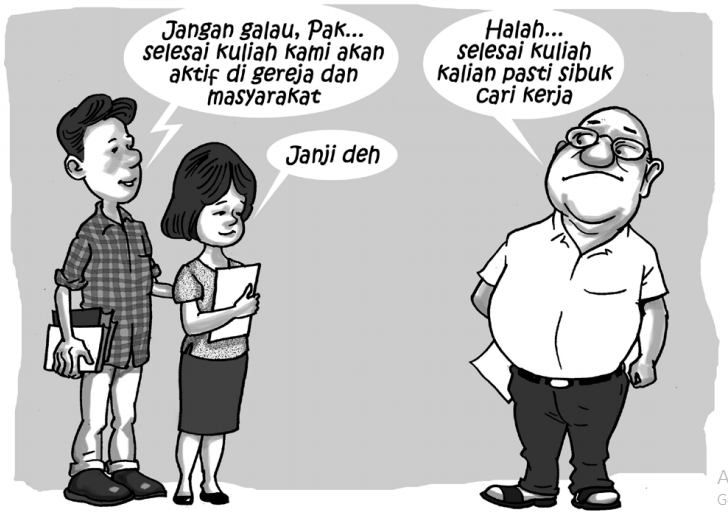
\includegraphics[scale=0.25]{BKL-2018-hari-1.png}
	\end{center}
\end{floatingfigure}

 \textit{\textbf{Tradisi Ibadat Katolik}} adalah tema BKL tahun 2018. Dalam konteks liturgi penting untuk menggali berbagai kekayaan budaya, adat kebiasaan, dan keariga lokal masyarakat yang selaras dengan iman Gereja. Tradisi ibadat Katolik dalam terang ajarang iman dan norma-norma liturgi Gereja perlu didalami agar kita semakin masuk dan mampu menghargai budaya setempat yang selaras dengan iman dan kitapun tetap kritis dan mampu merayakannya dengan baik dalam ibadat Katolik sesuai dengan norma-norma iman dan liturgi yang benar.

Pada hari ke-4 diangkat topik tentang Sakramen dan Sakramentali.

\textbf{Sakramen} berasal dari kata Latin \textit{sacramentum} yang
menerjemahkan   kata Yunani \textit{mysterion}.   Artinya,
"\textit{rencana keselamatan Allah yang terlaksana dalam
sejarah dan memuncak dalam diri Yesus Kristus}“.

\textbf{Sakramen} adalah tanda dan sarana yang
mengungkapkan karya dan tindakan Allah yang
menyelamatkan dan menjumpai kita melalui Yesus
Kristus dalam Roh Kudus

\textbf{Sakramentali} adalah \textbf{Tanda-tanda suci}, yang memiliki kemiripan dengan Sakramen-sakramen,     menandakan     kurnia-kurnia rohani yang diperoleh berkat doa
permohonan Gereja.

Perbandingan \textbf{sakramen} dan \textbf{sakramentali} adalah sbb:

\small
\begin{tabular}{|p{0.425\textwidth}|p{0.425\textwidth}|}
	\hline
	Sakramen & Sakramentali\\ \hline
	Daya guna \textit{ex opere operato}: menurut ritus (materia/-forma) yang dilakukan &
	Daya guna \textit{ex opere operantis}: menurut sikap batin orang yang merayakan\\ \hline
	Kristuslah pelaku utama dan pemberi rahmat sakramen &
	Yang utama adalah disposisi batin para pelaku sakramentali \\ \hline
	Pelayan: harus tertahbis & Pelayan: tidak harus tertahbis (imam) \\ \hline
\end{tabular}	
\normalsize


\subsection*{Ziarah ke Sendangsono}
Ziarah dilaksanakan pada tanggal 27 Mei 2017 dengan panitia diketuai oleh Bapak Heru Pratomo. Perjalanan dilakukan dengan menggunakan 8 mobil milik umat St. Theresia dengan peserta sejumlah 46 orang. Berangkat kira-kira jam 7 pagi dan kurang lebih 1 jam kemudian sudah sampai tujuan.

Sendangsono berada di Bukit Menoreh dan masuk dalam paroki St. Maria Lourdes Promasan. Keberadaan Sendangsono tak luput dari peran Romo Van Lith SJ, rohaniawan Belanda yang lama tinggal di Pulau Jawa. Hal itu juga menandakan bahwa Sendangsono tidak bisa dilepaskan dari lingkaran sejarah Gereja Katolik di Pulau Jawa mengingat Romo Van Lith sendiri merupakan salah satu rohaniwan yang menyebarkan ajaran Katolik di Pulau Jawa.

Pada 14 Desember 1904 silam Romo Van Lith membaptis 171 warga setempat dengan air dari kedua pohon sono, termasuk Barnabas sebagai katekumen pertama. 25 tahun kemudian, tepatnya 8 Desember 1929, Sendangsono dinyatakan resmi menjadi tempat penziarahan oleh Romo JB Prennthaler SJ.

Ziarah kali ini dilakukan dengan mengambil rute yang menuju langsung ke dekat sendang. Oleh karena itu peziarah St. Theresia hanya melakukan jalan salib yang rute pendek. Selesai jalan salib ternyata masih sempat mengikuti misa di sendang. Selesai misa dan istirahat sejenak, peziarah pulang dan sampai rumah sekitar jam setengah dua.


\subsection*{Komuni Pertama}
Komuni pertama untuk Lintang (Maria Lintang Novianti) di Gereja Marganingsih Kalasan pada tanggal 3 Juni 2018. Dari stasi Maguwo ada 20 penerima komuni pertama.

Tanggal 7 Juni 2018 bertepatan dengan doa lingkungan diserahkan kenang-kenangan kepada Lintang. Kenang-kenangan yang berupa buku-buku rohani diserahkan oleh Ketua Lingkungan.

\subsection*{Pernikahan mBak Vita}

\subsection*{BKSN 2018}

\subsection*{Penerimaan Sakramen Penguatan}

\subsection*{Peringatan 2 tahun meninggalnya Ibu Theresia Suci Wahyuningsih}


\subsection*{Ziarah ke Sendang Ratu Kenya Wonogiri}

\subsection*{Pesta Nama dan Penutupan Bulan  Rosario}

\subsection*{Adven}
	
\subsection*{Jagong Bayi Yesus}
